
%--------------------------------------------------------------------------
% THESIS: The MAIN thesis file from which all other things are included.
%--------------------------------------------------------------------------

% Include the header which includes packages, the Acadia style and definitions.

%---------------------------------------------------------
% Header: This file includes all the packages and custom definitions
% we have used in this example thesis.
%----------------------------------------------------------

% Uncomment the following line if, for some reason, you want a PDF 1.4
% document, rather than (at time of writing) PDF 1.5.
% \pdfminorversion=4

\documentclass[12pt,twoside,openright]{report}

% With these lines, when one tried to copy/paste from AR it does The
% Right Things for ligatures.
\input{glyphtounicode}
\pdfgentounicode=1

%---------------------
% START: Packages
%---------------------
\usepackage{textcomp}
\usepackage[latin1]{inputenc}
\usepackage{amsmath}
\usepackage{amsfonts}
\usepackage{amssymb}
\usepackage{amsthm}
\usepackage{graphicx}
\usepackage{soul}
\usepackage{listings}
\usepackage{subfig}
\usepackage{verbatim}
\usepackage{alltt}

% There are used in the graphics chapter.
% You can delete the following two lines if you use no tikz/pgf graphics
% in your thesis.
\usepackage{tikz}
\usepackage{pgfplots}

% Load the natbib citation package: set the citations to be numerical
% with square brackets separated by commas.
\usepackage[numbers,square,comma]{natbib}

% Now include the Acadia thesis style
\usepackage{acadia-hon-thesis}

% Load the hyperref package.
% The options tell it to (a) use hyper-links to pages with Roman
% numerals that are different than pages with Arabic numbers, and
% (b) tell Adobe reader to show a page number matching the thesis page
% number (rather than sequentially numbering the PDF pages from 1).
\usepackage[plainpages=false,pdfpagelabels]{hyperref}

% The information in the first three lines here goes into the PDF
% document properties.
% The rest of the lines define options related to hyper-links.
% colorlinks: typeset links in the given colours
%	      (otherwise an ugly box is drawn around the links, although
%	       it is only seen on the screen, not in printed copies)
% A newer option (since May 2011) would be to just use the hidelinks option.
% Note: pdfprintscaling=None should discourage Adobe reader from wanting to
% scale your pages to fit printable area when you print from Adobe reader.
\hypersetup{%
    pdftitle={An investigation of Network Time Protocol},
    pdfauthor={Hanjie Li},
    pdfkeywords={NTP, algorithm, time},
    colorlinks = true,
    linkcolor = black,
    anchorcolor = black,
    citecolor = black,
    filecolor = black,
    urlcolor = black,
    pdfprintscaling=None
}


% Load the algorithm/mic packages and use chapter-wise numbering
\usepackage[chapter]{algorithm}
\usepackage{algorithmic}


% JD addition:
% The url package does not, by default, allow breaks at '-'.  Change this
% by adding \do\- to this macro.  If you don't want breaks at '-' in URLs,
% just comment out or delete these lines:
\def\UrlBreaks{\do\.\do\@\do\\\do\/\do\!\do\_\do\|\do\;\do\>\do\]\do\-%
               \do\)\do\,\do\?\do\'\do+\do\=\do\#}%


%---------------------
% END: Packages
%---------------------
%\bibliographystyle{alpha}     % Make citations look like [Smi91], not [12]
\bibliographystyle{plainnat}   % Default boring and almost useless number.

% The depth of the table of contents: change the MAXIMUM depth of
% citations in your table of contents.
\setcounter{tocdepth}{6}

%
% Some definitions of commands used in this thesis
%

% For instance, if you have an acronym you like to use, then define a
% command, it's faster and if the acronym changes you only have to
% change it in one place.
\def\sysacro{SPECIALACRONYM}

% Allow us to change the margins easily and at will
\newenvironment{changemargin}[2]{%
  \begin{list}{}{%
    \setlength{\topsep}{0pt}%
    \setlength{\leftmargin}{#1}%
    \setlength{\rightmargin}{#2}%
    \setlength{\listparindent}{\parindent}%
    \setlength{\itemindent}{\parindent}%
    \setlength{\parsep}{\parskip}%
  }%
  \item[]}{\end{list}}

%setup the default format of listings
\lstset{
    basicstyle=\footnotesize,
    numbers=left,
    xleftmargin=5mm,
    linewidth=\textwidth,
    breaklines,
    frame=tb,
    frameround=fttt
}

% A new definition style
\newtheoremstyle{defstyle}	% name
    {3pt}			% Space above
    {3pt}			% Space below
    {}				% Body font
    {}				% Indent amount
    {\itshape}			% Theorem head font
    {:}				% Punctuation after theorem head
    {.5em}			% Space after theorem head
    {}		% Theorem head spec (can be left empty,meaning 'normal�)
\theoremstyle{definition}
\newtheorem{definition}{Definition}[chapter]


% Change comment style for algorithms
\renewcommand{\algorithmiccomment}[1]{/*#1*/}
% Change Require: to Input: for algorithms
\renewcommand{\algorithmicrequire}{\textbf{Input:}}
% Change Ensure: to Output: for algorithms
\renewcommand{\algorithmicensure}{\textbf{Output:}}


\begin{document}
    % PRELIMINARIES: This is the file you will use to setup your
    % name, date, advisor, etc. 
    %---------------------------------------------------------
% Preliminaries: Set up your own details in this file!
%----------------------------------------------------------

% Don't forget to remove the ()s in ALL of these "personalization" lines.

\title{An investigation of Network Time Protocol}
\author{Hanjie Li}
\dept{Computer Science}   % E.g., Physics, Computer Science,
\deptOrSchool{School}         % Pick one, remove the rest
\degree{Computer Science}  % E.g., Science, Arts, ...

\submissionMonth{March}	    % OR WHATEVER MONTH YOU ACTUALLY SUBMIT IN
\submissionYear{2019}
\copyrightYear{2019}		    % Probably the same as submissionYear.

% Use a "~" after the "r." of "Dr." so that TeX doesn't think you have
% ended a sentence (at which point it gives extra space).
\supervisor{Dr.~James Diamond}

% Remove the '%' from the next line and fill in the name if desired.
\cosupervisor{Dr.~Haiyi Zhang}

\headOrDirector{Dr.~Darcy Benoit}
% If the head or director is an ``acting'' head or director, uncomment
% the next line (i.e., delete the '%'):
% \justActing

% You will have to ask around to find out the name of the person
% to put here... it changes from year to year.
\honoursCommittee{Dr.~Joseph Hayes}
% https://research.acadiau.ca/Undergraduate_Student_Honours_Research.html

%-------------------------------------------------------------------------

% This outputs the title page, the approval page and the copyright page.
\firstThreePages

%-------------------------------------------------------------------------
% Now write your acknowledgements (if any).
% If you wish to acknowledge no-one, delete or comment-out the
% next few lines.

\Acknowledgments

Place any acknowledgments you might want to make here.

\noindent
Don't forget to be formal and professional.

%-------------------------------------------------------------------------

% This outputs the table of contents, lists of figures, tables, ...

\tocAndSuch

%-------------------------------------------------------------------------

\prefacesection{Abstract}

Time is widely used in life. Most people want to accurately know the time. If
we have a mechanical watch, maybe it is sufficient to make it accurate to one
second. However, on computers, especially on computers with high speed CPUs and
networks, people want their system time to be more accurate.  Time is sensitive
for some programs, such as logging programs or a program related to stock
market transactions. The Network Time Protocol is designed to synchronize
computers' system times. The basic idea is to let a computer communicate with
servers whose system times are synchronized, then based on the response, the
computer can change its system time. There are some atomic clocks which are
extremely accurate. Some servers can synchronize to them, and more servers can
synchronize to synchronized servers. The servers become a network.  When we
want to synchronize our computer, we can try to synchronize to servers in the
network.  The difficulty is we do not know how long a request packet takes to
travel from us to servers, how long it takes for a server to deal with the
request and how long a response packet takes to travel back to us.  This thesis
is going to investigate the algorithms of the Network Time Protocol to
determine and clearly document how  these problems are solved.

%-------------------------------------------------------------------------

% Don't mess with this line!
\afterpreface


    % CHAPTER CONTENT START
    % Replace all the lines from here down to ``CHAPTER CONTENT END''
    % with a collection of ``\include{XYZ}'' lines, where each such XYZ
    % is the name of a text file holding (for example) one chapter of
    % your thesis.
    % If you have appendices you need that ``\appendix'' line BEFORE
    % you \include your appendices.
    % introduction.tex

% why it is important
% why it is hard
% the increasing requirement of accurate time 
% computer clock structure

\chapter{Introduction}
Most computers and smartphones has their system times. Different accuracies are
required for different purposes. 
Assume that there is someone need to join a conference on time, and she can
only get time from her computer. If there the system time of the computer is
few minutes off compare with ``correct'' time, it is acceptable. But if the
offset amount is one hour, she will be there either too early and have to
wait for one hour or too late and the conference may be over at that time.

In some other cases, a very high accuracy of system time is required. For
example, there is a system handles stock market buy and sell orders. Generally,
more than one devices are there in the system. So that the system times among
devices should be ``the same'' since we need to know the order of the orders at
least. If the system is very busy and thousands orders may be created in one
second, every device should have system time accurate to millisecond at least.

As we can see in the previous example, only a ``local accuracy'' is required,
which means that every devices in the system need to synchronize its system
time to the same reference clock. If the reference clock is in an internal
device, they do not have to be synchronized to external devices. In some other
cases, a device may need to be synchronized to a standard time, such as UTC
(Coordinated Universal Time).  

The easy way of synchronizing clock is to ask someone else the time, and
adjust system clock manually. We always adjust the time of our
watches like that. The accuracy is quite enough if we do not need out watches
accurate to second. 

What about to imply this method on synchronizing computers system clock? Assume
computer A wants to synchronize to computer B, A can send a message to B then B
checks its time and replies to A. So A can adjust its system time.  
Obviously, there are a lot of problems.  The core one is that when A receive
the time, it can only know the time is when B checks its time. A cannot know
how long it is from then to when A receives the message. To solve these
problems, the network time protocol (NTP) is developed for devices to
synchronize their system times through network. 

\section{Computers' Clock}
\label{sec:computers_clock}
Different computers may use different hardware methods to maintain system time.
It relates to hardware architecture and operating system design. But they have
the same fundamental idea: increasing a counter with a ``constant'' frequency,
such as 1 GHz.
Based on the frequency and the counter, the system time can be calculated
when necessary. But in practice, the frequency is not constant. First of all,
there may be some manufacturing error, which makes it slightly different from
what it should be. Second, the frequency is affected by temperature, humidity
and so on. So the system clock can be very inaccurate if it has not been
synchronized for quite a long time, and the offset is unpredictable.

\section{Trend}
\label{sec:trend}
The performance of time synchronization is affected by the hardware
performance, the quality of network connection and the synchronization protocol
itself. 
As we have faster internet connection, and more powerful CPU, we have better
opportunity to get more accurate system clock. As we have more accurate system
clock, we can do more real-time stuff on internet. As we do more real-time
stuff on internet, we desire more accurate system clock. We always want to make
system clocks as accurate as possible after the improvements of internet
connection and CPUs. 

In real life, atomic clocks are considered the most accurate. In 2015 the most
accurate atomic clock is accurate to $2.1\times 10^{-18}$ second.
\cite{atomic_clock} % https://www.nature.com/articles/ncomms7896#introduction
This accuracy is far beyond CPU frequency and network latency. With this fact,
we can always improve the performance of time synchronization after we
significantly improve hardware or network connection.

    \chapter{Background}

\section{History and current situation}%
\label{sec:history_and_current_situation}
The basic idea of NTP has been there since early 1980s. NTP version 0 was
implemented in 1985, and it is documented in RFC-958. 
% But the actual implementation did a little bit more. 
The NTP packet header and the calculations of offset and delay are still being
used today. At that time, the nominal accuracy could be low tens of
milliseconds on an Ethernet and better than 100 milliseconds on paths spanning
the Atlantic.

NTP version 1 was documented in RFC-1059 one year later. It contains
specification of the protocol and algorithms.

NTP version 2 specification is documented in RFC-1119 in 1989. This version
includes new protocol for use in managing NTP servers and clients and
cryptographic authentication scheme.

At about the same time, another time synchronization protocol was presented,
which is Digital Time Synchronization Service (DTSS).

NTP version 3 specification appeared in 1992, following RFC-1305. This version
combined the good ideas from both NTP and DTSS.

After that, Simple Network Time Protocol version 4 was documented in RFC-2030
in 1996. SNTP is used if user do not need the ultimate performance of NTP or
it is not justified.

The latest version of NTP follows RFC-5905, which is version 4 and presented in
2010.
% history.pdf

\section{Reference clocks}%
\label{sec:reference_clocks}
``A reference clock is some device or machinery that spits out the current
time''~\cite{reference_clock}.
% http://www.ntp.org/ntpfaq/NTP-s-algo.htm#Q-REFCLK
The most important thing for reference clock is its accuracy, it must be
synchronized to some time standard (usually UTC). If we want to synchronize a
device to UTC, it requires reference clocks as sources. Some of them are
available for many government dissemination services, includes:~\cite{redbook}
\begin{itemize}
    \item Global Positioning System (GPS) and Long-Range navigation (LORAN-C)
        systems
    \item WWV/H and WWVB radio time/frequency stations
    \item U.S. Naval Observatory (USNO) and National Institutes of Science and
        Technology (NIST\null, formerly the National Bureau of Standards [NBS])
        telephone modem services in the United States
    \item Similar systems and services in other country
\end{itemize}
Generally, we want all devices synchronized to UTC as well as reference clocks.
But in some case, we may just want all devices in a local area network
synchronized to a certain ``standard'' time such as the system time of a
certain device among them. In this case, no reference clock is in the subnet.
But we can consider the device which others are synchronized to as a reference
clock. 

\section{Adjusting system time}%
\label{sec:adjusting_system_time}
As mentioned in Section~\ref{sec:computers_clocks}, every computer should have
a constant frequency to increase the number in a counter then calculate system
time. However, in practice, the frequency may be nether accurate nor
consistent. In this case, even if at some time we synchronized the system time
to UTC or a reference clock, it will be inaccurate later. This fact make it
necessary to synchronize a device frequently.

When system clock is adjusted by NTP\null, both the time and the frequency
will be adjusted. NTP uses \verb|ntp_adjtime()| or \verb|adjtime()| to adjust
system time when the offset is small. The benefit of using them is that they
will synchronize the system time step by step over a period of time by
adjusting a small amount in one step and finally make it synchronized. In
this case, any running program which is sensitive to time, such as a logging
program, will only be slightly impacted. If we want to change system time
back for some amount, it will not make later things ``happened'' earlier in
the log. If we want to change system time forwardly, there will not be a gap
in the time line, where nothing happened during that time. However, if the
offset it big, NTP will also change the system time to another value.

% \section{Concepts}%
% \label{sec:concepts}

% (Note: should this part be here or somewhere else or no need?)



    % overview.tex

\chapter{Overview}
% Three kinds of devices.
NTP operates on three different kinds of devices: primary servers, secondary
servers and clients. Primary servers are directly synchronized to reference
clocks and provide service that other devices can synchronize to them.
Secondary severs are synchronized to other servers instead of reference clocks
and provide synchronization service. Clients are synchronized to other servers
but they do not provide synchronization to others.

\section{Protocol modes}%
\label{sec:protocol_modes}
NTP has three basic protocol modes: \emph{server/client}, \emph{symmetric}
and \emph{broadcast}. They are also called association modes. 
%(NOTE: I DID NOT FIND ANY DEFINITION OF ASSOCIATION!)
In the server/client variant, clients send requests to server for
synchronization, and servers handle the request and send response. We say
"clients pull synchronization from servers". The broadcast is like the
opposite mode of server/client mode, in which servers push synchronization to
clients. Symmetric mode is a combination of two server/client modes and two
broadcast modes. In symmetric variant, a peer operates as both client and
server and each peer both push and poll synchronization to and from each
other.~\cite{rfc5905}

There are two interleaved modes which we will discuss in
Section~\ref{sub:timestamps_in_ntp_packet}.

\section{Layered Network}
\label{sec:Layered_network}
The NTP network or subnet has a hierarchy architecture, which is divided into
several levels. Each level is called a stratum. All primary servers are in
stratum one, which is the highest stratum. Secondary servers are assigned the
stratum number one great than the server's stratum number which it synchronizes
to. E.g., if a secondary server synchronizes to a server in stratum 3, it is in
stratum 4. The maximum stratum number is 16.~\cite{rfc5905}
Typically, clients do not have stratum number, but we can treat them
as in a stratum by using the same rule as secondary servers.
As the stratum number increases, the accuracy of devices in stratum
decreases.

Figure~\ref{fig:layered_network} shows the basic structure of NTP subnets. The
arrows indicate the direction of synchronization. An arrow from server 3 to
server 1 indicates that server 3 communicates with server 1 and tries to
synchronize to it but server 3 may not actually synchronize to server 1.

% This figure is made by myself, may need improvement
% fig:layered_network
% figures/overview-layer.tex

\begin{figure}[htpb]
\begin{center}
\begin{tikzpicture}[scale=0.7, transform shape,
        squarednode/.style={rectangle, draw=black, very thick, minimum
        size=10mm, minimum width=20mm, align=center},
    ]
    % Nodes
    % reference clocks
    \node[squarednode]  (rc)                {Reference Clocks};
    % servers
    \node[squarednode]  (s2)      [below=of rc] {Server 2};
    \node[squarednode]  (s1)      [left=of s2]  {Server 1};
    \node[align=center] (lab1)    [left=10 mm of s1]  
                        {Stratum 1\\ (Primary Servers)};
    \node[align=center] (lab2)    [right=of s2] {\dots};

    \node[squarednode]  (s3)      [below=of s1] {Server 3};
    \node[squarednode]  (s4)      [below=of s2] {Server 4};
    \node[align=center] (lab3)    [below=12mm of lab1]  {Stratum 2};
    \node[align=center] (lab4)    [right=of s4] {\dots};

    \node[align=center, rotate=90] (lab5)    [below=10mm of lab3] {\dots};

    \node[align=center] (lab6)    [below=17mm of lab3]  {Stratum n};
    \node[squarednode]  (client)  [below=13mm of s3] {Client};
    
    % synchronizations
    \draw[-latex, thick] (s1) -- (rc);
    \draw[-latex, thick] (s2) -- (rc);
    \draw[-latex, thick] (s3) -- (s1);
    \draw[-latex, thick] (s3) -- (s2);
    \draw[-latex, thick] (s4) -- (s2);
    \draw[-latex, thick] (client) -- (s2);
    \draw[-latex, thick] (client) -- (s3);
    \draw[-latex, thick] (client) -- (s4);

\end{tikzpicture}
\end{center}
\caption{NTP Layered Network}
\label{fig:layered_network}
\end{figure}




% Feb 20 2019, Dr. Diamond gave some advise about this paragraph
As people want their devices to be accurate, it is better to synchronize to
primary servers. But this can make primary servers very busy. Based on the rule
of engagement for NTP users, ``clients should avoid using primary servers
whenever possible''. Even though, some busy primary servers have more than 700
clients. 
% http://support.ntp.org/bin/view/Servers/RulesOfEngagement
It is said that the synchronizations provided by secondary servers in stratum 2
are accurate enough for most end-users. And clients are suggested to use three
to five servers. In practice, there are some pools of secondary servers.
Clients can assign a pool as a server which they want to synchronize to. When
the pool receive the connection request, it uses DNS round robin to select a
random server from the pool. Then client actually connects to the selected
server.
% http://support.ntp.org/bin/view/Servers/NTPPoolServers

\section{Processes}
\label{sec:processes}
% Architecture of client processes.
As Figure~\ref{fig:architecture_overview} shows, operations of an NTP client
can be separated into the following processes:
\begin{itemize}
    \item Peer/poll Processes\\
        This part deal with communications between client and servers. It has
        poll processes and peer processes. Poll processes send requests to
        servers. Peer processes keep track of a set of statistics for every
        server.
    \item System Process\\
        System process has algorithms to do some filter and correction work to
        the statistics of all peers, then pass them to clock discipline
        process.
    \item Clock Discipline Process\\
        Clock discipline process is like a lowpass filter to smooth the data.
        This process also maintains the poll intervals.
        % red book p. 40
    \item Clock Adjust Process\\
        This part adjusts the system clock to make it continuous and monotonic
        approximately. 
        % red book p. 40
\end{itemize}
The structure of NTP is like a loop. It requests synchronization to servers, after
gets response, it deals with it then adjust system time. After that, there are some
feedback used to control poll processes.

In later chapters, we will discuss peer/poll processes and system process
separately, and discuss clock discipline process and clock adjust process
together. Note that, in NTP official documents, ``server'' and ``peer'' are
used interchangeably.

% This figure is made based on the figure from
% https://www.eecis.udel.edu/~mills/ntp/html/warp.html
% fig:architecture_overview
% overview-arch.tex

%\begin{figure}[htpb]
%    \centering
%    \includegraphics[width=0.8\linewidth]{../figures.old/fig_3_1.png}
%    \caption{NTP architecture overview}
%    \label{fig:arch_overview}
%\end{figure}


\begin{figure}[htpb]
\begin{center}
\begin{tikzpicture}[scale=0.7, transform shape,
        squarednode/.style={rectangle, draw=black, very thick, minimum
        size=15mm, minimum width=30mm, align=center},
        squarednode1/.style 2 args={draw=black, very thick, minimum
        size=15mm,fit={(#1.north) (#2.south)}, text width=, inner sep=2mm, text
        centered, align=center},
        circlenode/.style={circle, draw=black, very thick, minimum size=15mm},
        border/.style={-, draw=black, very thick, dashed},
    ]
    % Nodes
    % remote servers, peer/poll process
    \node[squarednode]  (s1)                {Server 1};
    \node[squarednode]  (s2)  [below=of s1] {Server 2};
    \node[squarednode]  (s3)  [below=of s2] {Server 3};
    \node[align=center](lab1)[below=of s3] {Remote\\ servers};

    \node[squarednode]  (p1)  [right=of s1] {Peer/poll 1};
    \node[squarednode]  (p2)  [right=of s2] {Peer/poll 2};
    \node[squarednode]  (p3)  [right=of s3] {Peer/poll 3};
    \node[align=center](lab2)[below=of p3] {Peer/Poll\\ processes};

    \draw[border] ($(p1.north west) + (-0.4, 0.2)$) -| ($(lab2.south east) +
    (0.8, -0.2)$);
    \draw[border] ($(p1.north west) + (-0.4, 0.2)$) |- ($(lab2.south east) +
    (0.8, -0.2)$);

    % system process
    \node[squarednode]  (sa1) [right=of p2]
    {Selection\\ and\\ clustering\\ algorithms};
    \node[squarednode] (sa2) [right=of sa1] {Combine\\ algorithms};
    \node[align=center](lab3)[above=5mm of sa2] {System\\ process};

    \draw[border] ($(lab3.north east) + (1.0, 0.2)$) -| ($(sa1.south west) +
    (-0.4, -0.8)$);
    \draw[border] ($(lab3.north east) + (1.0, 0.2)$) |- ($(sa1.south west) +
    (-0.4, -0.8)$);

    % clock discipline process
    \node[squarednode] (lf) [right=of sa2] {Loop filter};
    \node[align=center](lab4)[above=5mm of lf] {Clock discipline\\ process};
    \draw[border] ($(lab4.north east) + (0.3, 0.2)$) -| ($(lf.south west) +
    (-0.4, -0.8)$);
    \draw[border] ($(lab4.north east) + (0.3, 0.2)$) |- ($(lf.south west) +
    (-0.4, -0.8)$);

    % clock adjust process
    \node[circlenode] (vfo) [below=25mm of lf] {VFO};
    \node[align=center](lab5)[below=5mm of vfo] {Clock adjust\\ process};
    \draw[border] ($(vfo.north east) + (1.0, 0.5)$) |- ($(lab5.south west) +
    (-0.2, -0.2)$);
    \draw[border] ($(vfo.north east) + (1.0, 0.5)$) -| ($(lab5.south west) +
    (-0.2, -0.2)$);
    
    % Lines
    % server-peer/poll process
    \foreach \x/\y in {s1/p1, s2/p2, s3/p3} {
        %\draw[-] (\x) -- (\y);
        \draw[-latex, thick] ($(\x.north east)!0.5!(\x.east)$) --
        ($(\y.north west)!0.5!(\y.west)$); 
        \draw[latex-, thick] ($(\x.south east)!0.5!(\x.east)$) --
        ($(\y.south west)!0.5!(\y.west)$); 
    }
    % peer/poll process
    \draw[-latex, thick] (p2.north) -- (p1.south);
    \draw[-latex, thick] (p3.north) -- (p2.south);
    % peer/poll process-system process
    \draw[-latex, thick] (p1.east) -- (sa1.north west);
    \draw[-latex, thick] (p2.east) -- (sa1.west);
    \draw[-latex, thick] (p3.east) -- (sa1.south west);
    % system process
    \draw[latex-, thick] (sa2.west) -- (sa1.east);
    % system process-clock discipline process
    \draw[-latex, thick] (sa2.east) -- (lf.west);
    % clock discipline process-clock adjust process
    \draw[-latex, thick] (lf.east) -- ($(lf.east) + (1,0)$) |- (vfo.east);
    % clock adjust process-poll process
    \draw[-latex, thick] (vfo.west) -| (p3.south);
    

\end{tikzpicture}
\end{center}
\caption{NTP architecture overview}
\label{fig:architecture_overview}
\end{figure}




% (What is the stuff I want to add here when I was taking shower on Fer 5?)


    % peer_poll.tex
\chapter{Peer/Poll Processes}
\label{cha:peer/poll_processes}

\section{Concepts}%
\label{sec:peer/poll_concepts}
\begin{enumerate}
    \item Offset $\theta$\\
        The maximum-likelihood time offset of the server clock relative to the
        system clock. This concept describes how different the client's time
        and the server's time are.
        % $$\theta_{AB} = \frac{1}{2}\left[\left(T_{i-2} - T_{i-3}\right) +
        % \left(T_{i-1} - T_i\right)\right]$$
    \item Delay $\delta$\\
        The round-trip delay between the client and server. It is equal to the
        time that a massage travels from the client to the server and the time
        it comes back.
        % $$\delta_{AB} = \left(T_{i} - T_{i-3}\right) - \left(T_{i-1} -
        % T_{i-2}\right)$$
    \item Dispersion $\varepsilon$\\
        The maximum error inherent in the measurement.
        Another definition: Potential clock offset error due to the maximum
        uncorrected system clock frequency error.
        These definitions are in some respect confused, we will discuss it with
        more detail in Section~\ref{sec:peer_processes}.
        % from website https://www.eecis.udel.edu/~mills/ntp/html/stats.html
    \item Jitter $\varphi$
        TODO: add this
\end{enumerate}

\section{Overview}%
\label{sec:peer_poll_overview}
Figure~\ref{fig:peer_poll_processes} shows the basic architecture of peer/poll
processes. The communication between client and server uses on-wire protocol,
which can provide sample statistics ($\theta_0, \delta_0, t_0$ in the figure).
The recent eight samples are stored in a shift register, with one more sample
statistic added ($\varepsilon$).  Then peer process applies clock filter
algorithm, which generates peer statistics ($\theta, \delta, \varepsilon,
\varphi$ in the figure), and passes them to system process.


% figures/peer_poll_figure.tex

\begin{figure}[htpb]
\begin{center}
\begin{tikzpicture}[scale=0.7, transform shape,
        squarednode/.style={rectangle, draw=black, very thick, minimum
        size=10mm, minimum width=20mm, align=center},
        border/.style={draw=black, dashed, very thick},
    ]
    % Nodes
    % server
    \node[squarednode]  (s)                {Server};

    % on-wire protocol
    \node[align=center] (onwire) at ($(s.east) + (2.5, 2)$) {On-wire Protocol};
    \draw[border] ($(onwire.north west) + (-0.2, 0.2)$) -|
            ($(onwire.north east) + (0.2, -5)$) -|
            ($(onwire.north west) + (-0.2, 0.2)$);
    % poll process
    \node[squarednode] (poll) at ($(onwire) + (0, -6)$) {Poll Process};
    \draw[-latex, thick] (poll) |- ($(s.south) + (0, -0.5)$) -- (s);

    % shift registers
    \node[squarednode] (sr) at ($(onwire) + (4.5,-2)$) 
            {Shift Registers\\
            $(\theta_1, \delta_1, \varepsilon_1, t_1)$\\
            $(\theta_2, \delta_2, \varepsilon_2, t_2)$\\
            $(\theta_3, \delta_3, \varepsilon_3, t_3)$\\
            $(\theta_4, \delta_4, \varepsilon_4, t_4)$\\
            $(\theta_5, \delta_5, \varepsilon_5, t_5)$\\
            $(\theta_6, \delta_6, \varepsilon_6, t_6)$\\
            $(\theta_7, \delta_7, \varepsilon_7, t_7)$\\
            $(\theta_8, \delta_8, \varepsilon_8, t_8)$
            };
    \draw[-latex, thick] (s) -- (sr) node[midway, above] 
            {$(\theta_0, \delta_0, t_0)$};
    % clock filter algorithm
    \node[squarednode] (cf) [right=of sr] {Clock Filter\\ algorithm};
    \draw[-latex, thick] (sr) -- (cf);

    % peer process
    \node[align=center] (peer) [below=2mm of sr.south east] {Peer Process};
    \draw[border] ($(sr.north west) + (-0.5, 0.2)$) -- 
            ($(sr.south west) + (-0.5, -1.2)$)
            -|
            ($(cf.east) + (0.2, 0)$) |-
            ($(sr.north west) + (-0.5, 0.2)$);


    % system process
    \node[squarednode] (sp) [right=2.5 of cf] {System process};
    \draw[-latex, thick] (cf) -- (sp) node[midway, above] 
            {$(\theta, \delta, \varepsilon, \varphi)$};
    
    % synchronizations
    % \draw[-latex, ultra thick] (s1) -- (rc);

\end{tikzpicture}
\end{center}
\caption{Peer/Poll processes}
\label{fig:peer_poll_processes}
\end{figure}



% fig:peer_poll_processes

The purpose of peer processes is to communicate with servers and to keep
statistics of the communications which can be used to determine how reliable
the servers are. For poll processes, their jobs are to manage the
communications to get sufficient data without making the servers too busy.

\section{On wire protocol}%
\label{sec:on_wire_protocol}
In NTP subnet, a client can send request to server and the server sends back
response after it got the request. The whole round of the communication can
generate a sample. For every sample, the client wants to know the difference
between the server's system clock and its, aka offset.
But it may take a while for the server to give the response. And it is not
predictable, as well as the network delay between the two devices.
In NTP subnet, clients and servers communicate under on-wire protocol. It
provides a smart way to calculate offset and delay for every sample. 

\subsection{Statistics calculation}%
\label{sub:statistics_calculation}
Figure~\ref{fig:on_wire1} represents the timestamps and communications between
a client and a server. The vertical dash line indicates the same time. The
arrow indicates the communication packets sent from one side and received at
the other side. The notation $T_i$ stands for the timestamp gotten from the
system clock of one device. 

% figures/on_wire1.tex

\begin{figure}[htpb]
\begin{center}
\begin{tikzpicture}[scale=0.7, transform shape,
        textnode/.style={rectangle, very thick, minimum
        size=10mm, minimum width=20mm, align=center},
        border/.style={draw=black, dashed, very thick},
        arrow/.style={-latex, ultra thick},
    ]
    % server
    \node[textnode]  (s)                {Server};
    \draw[arrow]     (s) -- ($(s) + (10,0)$);

    % client
    \node[textnode]  (c)    [below=20mm of s]            {Client};
    \draw[arrow]     (c) -- ($(c) + (10,0)$);

    % communications
    \draw[arrow]     ($(c) + (5, 0)$) -- ($(s) + (6, 0)$);
    \draw[arrow]     ($(s) + (8, 0)$) -- ($(c) + (9, 0)$);

    % vertical line
    \draw[border]    ($(s) + (3, 1)$) -- ($(c) + (3, -1)$);

    % labels
    \node[textnode] at ($(c) + (2.5, -0.5)$)   {$t_0$};
    \node[textnode] at ($(s) + (2.5, 0.5)$)    {$t_1$};
    \node[textnode] at ($(c) + (5, -0.5)$)   {$t_2$};
    \node[textnode] at ($(s) + (6, 0.5)$)    {$t_3$};
    \node[textnode] at ($(s) + (8, 0.5)$)    {$t_4$};
    \node[textnode] at ($(c) + (9, -0.5)$)   {$t_5$};

\end{tikzpicture}
\end{center}
\caption{Time stamps}
\label{fig:on_wire1}
\end{figure}



% fig:on_wire1

In ideal situation, if we have $T_1$ and $T_0$, which are timestamps gotten
from both devices at the same time, then we can get the offset $\theta$:
$$\theta = T_1 - T_0$$
But we cannot do this since we cannot determine whether two timestamps were
token at the same time. The on-wire protocol actually calculates the offset in
an alternative way:
\begin{equation}
    \theta = \frac{1}{2}\left[(T_3 - T_2) + (T_4 - T_5)\right]
    \label{eq:offset_def}
\end{equation}
Note that this equation is equivalent to:
$$\theta = \frac{T_3 + T_4}{2} - \frac{T_2 + T_5}{2}$$
which means that the offset is equal to the difference between two timestamps
which are the middle points of $T_3, T_4$ and $T_2, T_5$. 
If the network delay is symmetric, which means the time for packets to travel
from client to server and the time for packets to get back are equal, the
middle points are at the same time. In this case, it is equivalent to the ideal
situation. If the delay is asymmetric, there will be an error of the
calculation. This error is impossible to be corrected. However, there is one
scenario that the error can be attenuated.~\cite{redbook} We will discuss this
part in Section~\ref{sub:huff_n_puff_filter}.

The delay $\delta$ is calculated by:
\begin{equation}
    \delta = (T_5 - T_2) - (T_4 - T_3)
    \label{eq:delay_def}
\end{equation}
It is actually a difference of two time periods. It is not impacted by the
offset, since each time period is calculated using two timestamps from the same
device.
(NOTE: add the impact of frequency offset.)

There is another statistic $t$ in Figure~\ref{fig:peer_poll_processes}, which
indicates the time that the offset $\theta$ and delay $\delta$ are calculated.
In practice we can let $t = T_5$, because it is just used to indicate the order
of groups of sample statistics, we do not need it to be extremely accurate.
It is maintained by clock-adjust process. It counts the seconds since the
service was started.
In Figure~\ref{fig:peer_poll_processes}, we add subscript 0 to distinguish the
new group of samples statistics and the groups which are in the shift register.

\subsection{Timestamps in NTP packet}%
\label{sub:timestamps_in_ntp_packet}
% how to store timestamps and modes
% https://www.eecis.udel.edu/~mills/onwire.html
NTP uses NTP packets in communications. The NTP packet is a UDP
datagram.~\cite{rfc5905} There are four timestamps in NTP packet header:
\begin{enumerate}
    \item Reference Timestamp\\
        Time when the system clock was last set or corrected.
    \item Origin Timestamp (\emph{org})\\
        Time at the client when the request packet departs from it.
    \item Receive Timestamp (\emph{rec})\\
        Time at the server when the request packet is receive by it.
    \item Transmit Timestamp (\emph{xmt})\\
        Time at the server when the response packet departs from it.
\end{enumerate}
In peer process, we are interested in another one: destination
timestamp(\emph{dst}), which is the time at the client when it receives the
response packet. And the reference timestamp is not interested here. In
Figure~\ref{fig:on_wire1}, the packet leave at $T_4$ contains $T_4, T_3$ and
$T_2$ in its header, where
$$ org = T_2,~rec = T_3,~xmt = T_4 $$
When the client gets the packet, it captures $dst = T_5$.

The purpose of on-wire protocol is to calculate offset $\theta$ and delay
$\delta$ based on the communication. The four timestamps used in
Equation~\ref{eq:offset_def} and Equation~\ref{eq:delay_def} are important,
which are \emph{org}, \emph{rec}, \emph{xmt} and \emph{dst}.
High accuracy requires that they are captured as close to the actual time of
the relative event (sending or receiving packet) as possible. On-wire protocol
provides two interleaved modes which are \emph{interleaved symmetric} and
\emph{interleaved broadcast}. They are extensions of basic symmetric mode and
basic broadcast mode.~\cite{on_wire} 
%
In basic modes, \emph{org} and \emph{xmt} in outgoing packet are captured
before the packet is made, which is not the timestamp when the packet is sent. 
This kind of timestamps are called \emph{softstamps}. In this case, 
after softstamp is captured, there are something else to do before sending the
packet, such as add validation information to the packet and adding the packet
to the output queue, then the packet will wait in the queue before it is sent.
For \emph{rec} and \emph{dst}, which are also called \emph{drivestamps}, they
are captured ``shortly after the input device interrupt and before adding the
buffer to the input queue''.\cite{on_wire} We can see that the drivestamps are
more accurate than softstamps because there is only a short delay by handling
the interrupt. If we can capture timestamps exactly when packets are sent or
received, they will be more accurate. However, we need additional hardware
support to do this.

In interleaved modes, we can make softstamps more accurate without
additional hardware support. The trade off is that we need more packets.
Instead of capturing softstamps before the packets are made, we can capture
them shortly after the output interrupt. In this case, the accuracy is similar
with drivestamps but they can not be sent in the very packets which they
represent the time they are sent. We need one more packet if we want to send
softstamps. More detail about interleaved modes are beyond the scope of this
thesis.

\subsection{Non-reliable protocol}%
\label{sub:non_reliable_protocol}
As mentioned in Section~\ref{sub:timestamps_in_ntp_packet}, the NTP packet is a
UDP datagram. This make on-wire protocol not reliable, which means that there
is no guarantee about the packet. Reliable delivery actually decreases the
reliability of NTP packet. Assume we are implementing on-wire protocol to make
it reliable by using similar technique like TCP, a lost packet will be sent
again. However, an identical packet is not valid since the timestamp which
indicates the time when the packet is sent is incorrect.

\section{Peer processes}%
\label{sec:peer_processes}
For each server, on-wire protocol provides sample statistics $\theta, \delta$
and $t$ and passes them to peer process. Then the peer process maintains them
and the clock filter algorithm calculates peer statistics based on them.

\subsection{Sample statistics maintenance}%
\label{sub:sample_statistics_maintenance}
As mentioned in Section~\ref{sec:peer_poll_overview}, there is a shift register
which stores the recent eight samples. When a packet arrives, the peer process
replace the oldest sample by the new one with a dispersion $\varepsilon$ added.
The dispersion is initialized as:
$$ \varepsilon = \rho_r + \rho_s + \phi (T_5 - T_2) $$
Where 
\begin{itemize}
    \item 
        $\rho_r$ is the root precision in NTP packet. 
    \item 
        $\rho_s$ is the system
        precision which we will discuss in next chapter. (NOTE: REF HERE).
    \item
        $\phi = 15 ppm = 15 \mu s/s$ is a constant.
    \item
        $T_5$ and $T_2$ are the two timestamps in Figure~\ref{fig:on_wire1}. In
        other word, $T_5$ is \emph{dst} and $T_2$ is \emph{org}.
\end{itemize}
After storing the sample statistics into the shift register, the peer process
increases dispersion in a constant rate $\phi$.

In Section~\ref{sec:peer/poll_concepts} we mentioned that dispersion is the
maximum error. Now we can consider dispersion as a function of time ($t$) and
we have:
\begin{equation}
    \varepsilon(t) = \rho_r + \rho_s + \phi (t - T_2)
    \label{eq:dispersion}
\end{equation}
In Equation~\ref{eq:dispersion}, dispersion has two parts. $\rho_r + \rho_s$
represents the error due to the precisions of server and client clocks. $\phi
(t - T_2)$ represents the error due to frequency tolerance and time.
(TODO: add more about 15 ppm)

\subsection{Initial and invalid samples}%
\label{sub:initial_and_invalid_samples}
When the service starts, all eight samples in the shift register are
initialized to the dummy tuple: $\theta = 0, \delta = \verb|MAXDISP|,
\varepsilon = \verb|MAXDISP|, t = 0$, where $\verb|MAXDISP| = 16$ is the
maximum dispersion.~\cite{rfc5905} 

There is a 8-bit shift register called reach register which is shared by peer
and poll process and used to determine whether the server is reachable and the
data is fresh. It is maintained by poll process, which we will discuss in
Section~\ref{sec:poll_processes}. After a packet is sent to the server, the
register is shifted left by one bit and the rightmost bit is set to 0. If a
valid packet is arrived from the server, the rightmost bit is set to 1. A
server is reachable only when there is at least one non-zero bit in the
register. If the three rightmost bit are all 0, there will be a dummy tuple
inserted into the shift register of samples by replacing the oldest one which
indicates invalid sample.

\subsection{Clock filter algorithm}%
\label{sub:clock_filter_algorithm}
The clock filter algorithm calculates peer statistics used in system process.
As mentioned in Section~\ref{sec:peer_poll_overview}, there are 8 samples in
the shift register. Clock filter algorithm selects one of them represents the
offset and delay of the server, then calculates the dispersion and jitter,
passes them to the system process as well as the arrive time of selected
sample.

Figure~\ref{fig:clock_filter} is ``a wedge scattergram plotting sample points of
offset versus delay collected over a 24-hr period''. (NOTE: cite here) It shows
that with as the delay increases, the variance of offset increases as well. In
this case, the best sample should be the one with lowest delay. We will discuss
this more in Section~\ref{sub:huff_n_puff_filter}.

% clock_filter

\begin{figure}[htb]
    \centering
    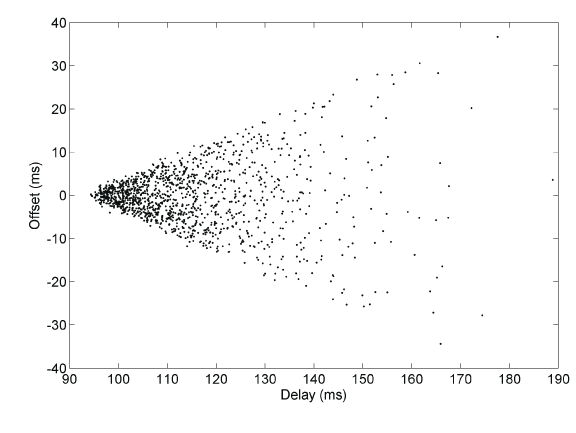
\includegraphics[width=0.5\textwidth]{figures/clock_filter.png}
    \caption{Wedge Scattergram}
    \label{fig:clock_filter}
\end{figure}


% fig:clock_filter

Based on the result we got from Figure~\ref{fig:clock_filter}, clock filter
algorithm first sort the samples by their delay. If the first sample is later
than the last sample we chose, it is selected, otherwise nothing more happen.
This mechanism guarantees that one sample will only be used at most once.

After the selection, the offset $\theta$ and delay $\delta$ of the sample
become peer statistics with the same names. The sorted samples are indexed from
0 to 7 from the one with the lowest delay to the one with highest. Here
$\varepsilon_i$ indicates the dispersion of the sample with index $i$. We
calculate peer dispersion $\varepsilon$ by:
\begin{equation}
    \varepsilon = \sum^{7}_{i=0} \frac{\varepsilon_i}{2^{(i+1)}}
    \label{eq:peer_dispersion}
\end{equation}
The peer jitter $\varphi$ is calculated by:
\begin{equation}
    \varphi = \sqrt{\frac{1}{n-1} \sum^{n-1}_{j=1} (\theta_0 - \theta_j)^2}
    \label{eq:peer_jitter}
\end{equation}
where $n$ is the number of valid samples in the shift register ($n > 1$).
The peer jitter is the root mean square (RMS) of difference between sample
offsets and the sample offset of selected sample, ``it represents the nominal
error in estimating the offset''~\cite{rfc5905}. A larger jitter indicates
that the offset varies more, which we can consider that there may be some
problem with the server and/or the connection, since the offset should not
change much if we did not adjust client's system clock by a large amount.

\subsection{Huff-n'-puff filter}%
\label{sub:huff_n_puff_filter}
Now we are going to look at Figure~\ref{fig:clock_filter} closely. In the
figure, ``there are two limb lines with at slope $\pm0.5$, representing the
limits of sample variation''. (NOTE: cite here) 
The variation of offset is caused by the asymmetric delay, and it is actually
an error.

Figure~\ref{fig:huff_n_puff1} shows the relationship between delay and offset
error.  Figure~\ref{subfig:best_case} shows the best case where the delays are
symmetric. In this case, the middle points which are indicated by the ends of
dash line (other two figures are the same) are at the same time. As we
mentioned in Section~\ref{sub:statistics_calculation}, the calculation in
Equation~\ref{eq:offset_def} is correct. 

% figures/huff_n_puff1.tex

\begin{figure}[htpb]
\begin{center}
\subfloat[Best case]{
\begin{tikzpicture}[scale=0.73, transform shape,
        textnode/.style={rectangle, very thick, minimum
        size=10mm, minimum width=20mm, align=center},
        border/.style={draw=black, dashed, very thick},
        arrow/.style={-latex, ultra thick},
    ]
    % server
    \node[textnode]  (s)                        {Server};
    \draw[arrow]     (s) -- ($(s) + (9,0)$);

    % client
    \node[textnode]  (c)    [below=20mm of s]   {Client};
    \draw[arrow]     (c) -- ($(c) + (9,0)$);

    % communications
    \draw[arrow]     ($(c) + (3, 0)$) -- ($(s) + (3.5, 0)$);
    \draw[arrow]     ($(s) + (6.5, 0)$) -- ($(c) + (7, 0)$);

    % dash line
    \draw[border]    ($(s) + (5, 0)$) -- ($(c) + (5, 0)$);
\end{tikzpicture}
\label{subfig:best_case}
}
\subfloat[Normal case]{
\begin{tikzpicture}[scale=0.7, transform shape,
        textnode/.style={rectangle, very thick, minimum
        size=10mm, minimum width=20mm, align=center},
        border/.style={draw=black, dashed, very thick},
        arrow/.style={-latex, ultra thick},
    ]
    % server
    \node[textnode]  (s)                        {Server};
    \draw[arrow]     (s) -- ($(s) + (9.5,0)$);

    % client
    \node[textnode]  (c)    [below=20mm of s]   {Client};
    \draw[arrow]     (c) -- ($(c) + (9.5,0)$);

    % communications
    \draw[arrow]     ($(c) + (3, 0)$) -- ($(s) + (4, 0)$);
    \draw[arrow]     ($(s) + (6, 0)$) -- ($(c) + (7.5, 0)$);

    % dash line
    \draw[border]    ($(s) + (5, 0)$) -- ($(c) + (5.25, 0)$);
\end{tikzpicture}
\label{subfig:normal_case}
}

\subfloat[Extremely asymmetric case]{
\begin{tikzpicture}[scale=0.7, transform shape,
        textnode/.style={rectangle, very thick, minimum
        size=10mm, minimum width=20mm, align=center},
        border/.style={draw=black, dashed, very thick},
        arrow/.style={-latex, ultra thick},
    ]
    % server
    \node[textnode]  (s)                        {Server};
    \draw[arrow]     (s) -- ($(s) + (10,0)$);

    % client
    \node[textnode]  (c)    [below=20mm of s]   {Client};
    \draw[arrow]     (c) -- ($(c) + (10,0)$);

    % communications
    \draw[arrow]     ($(c) + (3, 0)$) -- ($(s) + (3, 0)$);
    \draw[arrow]     ($(s) + (5, 0)$) -- ($(c) + (7.5, 0)$);

    % dash line
    \draw[border]    ($(s) + (4, 0)$) -- ($(c) + (5.25, 0)$);
    \draw[border]    ($(s) + (4, 0)$) -- ($(c) + (4, 0)$);

    % labels
    \node[textnode] at ($(c) + (3, -0.5)$)      {$T_0$};
    \node[textnode] at ($(s) + (3, 0.5)$)       {$T_1$};
    \node[textnode] at ($(s) + (5, 0.5)$)       {$T_2$};
    \node[textnode] at ($(c) + (7.5, -0.5)$)    {$T_3$};
    \node[textnode] at ($(s) + (4, 0.5)$)       {$T_4$};
    \node[textnode] at ($(c) + (5.25, -0.5)$)   {$T_5$};
    \node[textnode] at ($(c) + (4, -0.5)$)      {$T_6$};

\end{tikzpicture}
\label{subfig:extremely_asymmetric_case}
}
\end{center}
\caption{The relationship between delay and offset variance}
\label{fig:huff_n_puff1}
\end{figure}



% fig:huff_n_puff1

In Figure~\ref{subfig:normal_case}, it is the normal case, the delays are
slightly different, which makes the middle points slightly different as well.
This difference leads an error of offset.

In Figure~\ref{subfig:extremely_asymmetric_case}, it represents the extremely
asymmetric case, where there is no upload delay and the download delay is
relatively large. Assume $T_6$ and $T_4$ are captured in the same time, the
error of offset is the difference between $T_5$ and $T_6$. We can prove that it
is equal to $-\frac{1}{2}\delta$. In another case, if the upload delay is
relatively large and the download delay is zero, the error is equal to
$\frac{1}{2}\delta$. Note that these cases are the situations when the error is
maximum.

With this analysis, we know that the slope $\pm0.5$ is not determined by
experiment, but is calculated in theory and we know the variation of offset is
actually error, which is the reason that we select the sample with smallest
delay, which leads to smallest offset error.

The clock filter algorithm works best when there is a symmetric delay, as
Figure~\ref{fig:clock_filter} shows. It is also mentioned that the errors due
to asymmetric delay are almost unable to be corrected. However, huff-n'-puff
filter is used here to attenuate the errors.

Figure~\ref{fig:huff_n_puff2} shows the scattergram like
Figure~\ref{fig:huff_n_puff1}, but the network delay is much asymmetric. From
the figure, we find that the samples are close to the upper limb line, which
indicates that the offset error is positive. This means that the upload delay
is larger than the download delay. By applying huff-n'-puff filter, we can do
the following stuff:
\begin{itemize}
    \item 
        Remember the recent sample with lowest delay where ``recent'' usually
        means recent hours. The offset and delay of the sample are denoted by 
        $\theta_0$ and $\delta_0$. Note that the sample is near the apex.
    \item 
        For a coming new sample whose offset and delay are $\theta_i$ and
        $\delta_i$, we keep its delay value and adjust offset by:
        \begin{equation}
            \theta = 
            \begin{cases}
                \displaystyle
                \theta_i - \frac{\delta_i - \delta_0}{2}, &\text{ if }\theta_i
                > \theta_0\\
                \displaystyle
                \theta_i + \frac{\delta_i - \delta_0}{2}, &\text{ if }\theta_i
                < \theta_0\\
            \end{cases}
            \label{eq:huff_n_puff}
        \end{equation}
\end{itemize}

% figures/huff_n_puff2.tex

\begin{figure}[htb]
    \centering
    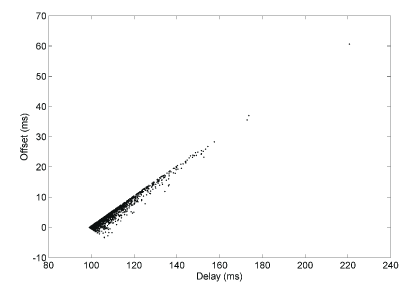
\includegraphics[width=0.8\textwidth]{figures/huff_n_puff.png}
    \caption{Huff-n'-puff Wedge Scattergram}
    \label{fig:huff_n_puff2}
\end{figure}


% fig:huff_n_puff2

Note that this adjustment is actually move the sample points close to the
vertical line which go through the point $(\delta_0, \theta_0)$, if the samples
are near the upper limb line, as Figure~\ref{fig:huff_n_puff2} shows. It is
also said that it is less effective and will lead to significant errors if a
large amount of samples are in the area between the limb
lines.~\cite{huff_n_puff} If the practice situation is like
Figure~\ref{fig:huff_n_puff2}, the adjustment works fine, since it can
avoid the variation of offset which can be considered as error.

%\subsection{Reachability detection}%
%\label{sub:reachability_detection}
% https://docs.ntpsec.org/latest/stats.html
% redbook

\section{Poll processes}%
\label{sec:poll_processes}
As mentioned in Section~\ref{sec:peer_poll_overview}, poll processes are
designed to control the interval of communications in order to get significant
data without making servers too busy. 

The key part of poll process it the time constant $T_c$ and its relative time
exponent $\uptau$ where $T_c = 2 ^ {\uptau}$. A client send poll request to
each server with a \emph{poll interval} of $T_c$ seconds. $\uptau$ is a whole
number and is called the \emph{poll exponent}, which ranges from 4 to 17 and is
maintained by the clock adjust process. 

$T_c$ and $\uptau$ are maintained by the clock discipline process, will discuss
it later in Chapter~\ref{cha:clock_discipline_process}.

(TODO: add burst, iburst, cite here)




    
% system_process.tex

\chapter{System Process}
\label{cha:system_process}

As mentioned in Section~\ref{sec:processes}, after peer/poll processes deal
with data from servers, the peer statistics are passed to the system process.
There are three algorithms in the system process:
\begin{itemize}
    \item Selection algorithm
    \item Clustering algorithm
    \item Mitigation algorithm
\end{itemize}

To understand the system process, we first introduce some concepts.

\section{Concepts}%
\label{sec:system_concepts}
\begin{enumerate}
    \item Truechimer and falseticker\\
        A truechimer is a clock that maintains timekeeping accuracy to a
        previously published (and trusted) standard, while a falseticker is a
        clock that does not.
    \item Root distance $\lambda$\\
        Root distance is a very important statistic used in system process, it
        ``represents the maximum error of the estimate due to all
        causes.''~\cite{performance_metrics} The root distance is calculated as
        the \emph{root delay} from the primary source of time plus the
        \emph{root dispersion} of that source. Here the source is the reference
        clock, the root delay and the root dispersion are similar with the
        statistics delay and dispersion we discussed in
        Chapter~\ref{cha:peer/poll_processes}, but relate to the source. We
        will discuss relative calculations in
        Section~\ref{sec:selection_algorithm}.
\end{enumerate}

(TODO: add purpose and figure of this part)

\section{Selection algorithm}%
\label{sec:selection_algorithm}
The selection algorithm takes peer statistics of each peer process then
determines truechimers among peers. The first thing is to calculate root
distance $\lambda$ for each peer.

\subsection{Root distance calculation}%
\label{sub:root_distance_calculation}

\begin{myverbbox}
    {\mindisp}MINDISP
\end{myverbbox}

As mentioned in Section~\ref{sec:system_concepts}, the root distance has two
parts: \emph{root delay} $\Delta$ and \emph{root dispersion} $E$. Furthermore, 
we have: 
\begin{equation}
    \Delta = \max(\mindisp, \delta_p + \delta)
    \label{eq:root_delay}
\end{equation}
and
\begin{equation}
    E = \varepsilon_p + \varepsilon + \varphi
    \label{eq:root_dispersion}
\end{equation}
Then we have root distance $\lambda$ which is calculated by:
\begin{align}
    \lambda & = \frac{\Delta}{2} + E\\
    & =\frac{\max(\mindisp, \delta_p + \delta)}{2} 
    + \varepsilon_p + \varepsilon + \varphi
    \label{eq:root_distance}
\end{align}
where 
\begin{itemize}
    \item $\mindisp$ is the minimum increment of dispersion.  It is used to
        avoid timing loops in NTP subnets with very fast processors and
        networks.~\cite{rfc5905} Its default value has three versions among
        official documents of NTP: 5 ms,~\cite{rfc5905} 10 ms,~\cite{rfc5905}
        and 1 ms.~\cite{performance_metrics}
    \item $\delta_p$ is the root delay of the peer, it is in the NTP packet
        header.
    \item $\varepsilon_p$ is the root dispersion of the peer, it is in the NTP
        packet header.
    \item $\delta$, $\varepsilon$ and $\varphi$  are the peer delay, peer
        dispersion and peer jitter we mentioned in
        Chapter~\ref{cha:peer/poll_processes}. Note that the peer dispersion
        $\varepsilon$ should be updated every time we access to it since it
        increases in a constant speed $\phi = 15 ppm = 15 \mu s/s$.
\end{itemize}

\subsection{Pre-selection checking}%
\label{sub:pre_selection_checking}
After the calculation of root distance for each peer, a number of checks are
performed, which includes the following checks:
\begin{enumerate}
    \item Stratum Error\\
        As we mentioned before, the stratum numbers are between 0 and 15
        inclusive. If the peer is never synchronized or its stratum number is
        not in the range, an stratum error occurs.
    \item Distance Error\\
        There is an option called \verb|MAXDIST| which by default is 1.5s for
        networks on the Earth and 2.5s for networks including the
        Moon.~\cite{clock_selection} (In the RFC file, its default value is
        1s~\cite{rfc5905}.)
    \item Loop Error\\
        If the peer is synchronized to the client, a loop error occurs.
    \item Unreachable Error\\
        If the server is Unreachable, an unreachable error occurs.
\end{enumerate}
If any one of the errors occurs, the relative peer is considered as
nonselectable and will not be considered in the following selection
algorithm.

\subsection{Background}%
\label{sub:selection_algorithm_background}

% correctness interval
For each peer, given the offset $\theta_i$ and the root distance $\lambda_i$,
we define a correctness interval of that peer: $[\theta_i - \lambda_i,
\theta_i + \lambda_i]$. By the definition of offset and root distance, if a
peer is a truechimer, we know that the true offset $\theta$ should be in the
interval, where the true offset is the offset of the reference clock relative
to the client.

In ideal situation that all peers are truechimers, and the reference clocks
that the peers synchronized to have very small amount of offsets among them,
the true offset should be in the intersection of all correctness intervals. In
practice, there may be some falsetickers, whose correctness intervals may have
two situations:
\begin{enumerate}
    \item The correctness interval of every falseticker has no intersection
        with the correctness intervals of all truechimers.\\ This is a good
        situation that we can determine falsetickers by correctness intervals.
    \item The correctness intervals of some falsetickers have intersection with
        the correctness intervals of all truechimers.\\ This is a bad situation
        that we cannot determine the falsetickers and the \emph{intersection
        interval} defined below will not contains the true offset.  However, we
        cannot do anything in this situation.
\end{enumerate}

Now we define the \emph{intersection interval} which is considered to contain
the true offset. The \emph{intersection interval} is the largest interval
which is subset of most correctness intervals. Note that the definition is
not the official one since it is considered to be confused.
Figure~\ref{fig:intersection_interval} shows an example of intersection
interval. There are four peers, which are also called candidates, A, B, C and
D. Their correctness intervals are the bars in the figure. As we can see,
there is no common intersection for all of them, but there is one for A, B
and C. In this case, candidate D is considered as a falseticker and the
intersection interval is indicated by the two dash lines which are the lower
and upper boundary of it.

% intersection_interval.tex


\begin{figure}[htpb]
\begin{center}
\begin{tikzpicture}[scale=0.7, transform shape,
        squarednode/.style={rectangle, draw=black, very thick, 
        align=center},
        border/.style={-, draw=black, very thick, dashed},
    ]
    % intervals
    \node[squarednode, minimum width=29mm] (b) {B};
    \node[squarednode, minimum width=35mm] (a) at ($(b.south) + (0.7, -1)$) {A};
    \node[squarednode, minimum width=50mm] (c) at ($(a.south) + (1.3, -1)$) {C};
    \node[squarednode, minimum width=20mm] (d) [left=15mm of c] {D};

    % boundary of intersection interval
    \coordinate (c1) at ( $(c.west) + (0, -1)$);
    \coordinate (b1) at ( $(b.west) + (0 , 1)$);
    \draw[border] (c1)node{} -- (c1 |- b1)node{};

    \coordinate (c2) at ( $(c.east) + (0, -1)$); 
    \coordinate (b2) at ( $(b.east) + (0 , 1)$);
    \draw[border] (b2)node{} -- (c2 -| b2)node{};

\end{tikzpicture}
\end{center}
    \caption{Intersection interval~\cite{clock_selection}}
\label{fig:intersection_interval}
\end{figure}


% fig:intersection_interval

\subsection{Selection algorithm}%
\label{sub:selection_algorithm}
The selection algorithms is used to cleave truechimers from falsetickers. It
does this by calculating the intersection interval given correctness intervals
from all candidates and "was devised by Keith Marzullo in his doctoral
dissertation.  It was first implemented in the Digital Time Synchronization
Service (DTSS) for the VMS operating system for the
VAX\null."~\cite{clock_selection}

Algorithm~\ref{alg:intersection_interval} shows how to get the intersection
interval.  In the algorithm, $endpoints$ is a list of tuples where each tuple
represents an endpoint of a correctness interval, it contains the id of the
peer, an integer $type$ to indicate whether it is the high($1$) or low($-1$)
endpoint of the correctness interval, and the $value$ of the endpoint. It is
initially empty.

\begin{algorithm}[ht]
    \centering
    \small
    \caption{Calculates the intersection interval.}
    \begin{algorithmic}[1]
        \REQUIRE
            correctness intervals.
        \ENSURE
            calculates the low and high endpoints of intersection interval.
        \STATE
            \COMMENT{initialization}
        \STATE
            $n \leftarrow 0, low \leftarrow 1e9, high \leftarrow -1e9$
        \FOR{$i \leftarrow$ correctness interval}
            \STATE
            Adds two tuples to $endpoints$
            \STATE
            $n \leftarrow n + 1$
        \ENDFOR
        \STATE
            Sorts $endpoints$ by the value.
        \STATE
        \STATE
            \COMMENT{Start calculation}
        \FOR{$allow \leftarrow \left[0, n/2 \right]$}
            \STATE
                \COMMENT{low points}
            \STATE
            $count \leftarrow 0$
            \FOR{$i \leftarrow \left[0, 2n \right]$}
                \STATE
                $low \leftarrow endpoints[i].value$
                \STATE
                $count \leftarrow count - endpoints[i].type$
                \IF{$count \geq n - allow$}
                \STATE
                    $break$
                \ENDIF
            \ENDFOR
            \STATE
            \STATE
                \COMMENT{high points}
            \STATE
            $count \leftarrow 0$
            \FOR{$i \leftarrow \left[2n, 0 \right]$}
                \STATE
                $high \leftarrow endpoints[i].value$
                \STATE
                $count \leftarrow count + endpoints[i].type$
                \IF{$count \geq n - allow$}
                    \STATE
                    $break$
                \ENDIF
            \ENDFOR
            \STATE
            \STATE
                \COMMENT{Check whether the intersection interval is found.}
            \IF{$high > low$}
                \STATE
                $break$
            \ENDIF
        \ENDFOR
    \end{algorithmic}
\label{alg:intersection_interval}
\end{algorithm}

Note that there are some details that we need to discuss. 
\begin{enumerate}
    \item 
        The initial values of $low$ and $high$ are not used unless the
        algorithm is called when there is no candidates.
    \item 
        The selection sort algorithm is used here to sort the list
        $endpoints$. It is not efficiency in principle, but it is acceptable
        here since there should not be hundreds of thousands of tuples to be
        sorted. In practice, each peer is manually assigned by the user of
        NTP, so even the number of tuples should be as twice as the number of
        peers, it will not be several hundreds. (Maybe no more than twenty.)
    \item
        The variable $allow$ indicates the number of falsetickers. From the
        algorithm, we can see that if we cannot get an intersection interval
        which is the intersection of more than half correctness intervals,
        the algorithm gives up and no truechimers can be
        found.~\cite{clock_selection}
    \item
        The algorithm first try to find an intersection of all correctness
        intervals. If it fails, it increase $allow$ by one, then try to find
        an intersection interval for one less correctness intervals. Then it
        repeats the step until an intersection interval is found or $allow$
        is to large.
\end{enumerate}
If the algorithm successfully ends, the truechimers left are used in the
clustering algorithm, otherwise nothing further happens.  The system clock of
the client will not be synchronized.

Note that the algorithm ``implementation'' in RFC5905 page 91 is completely
wrong.

\subsection{Midpoints of correctness intervals}
\label{midpoints_of_correctness_intervals}
(NOTE: finish this part after finishing this chapter)

\section{Clustering algorithm}%
\label{sec:clustering_algorithm}
For truechimers, we can  calculate the \emph{selection jitter} statistic for
each of them, where it is the root-mean-square (RMS) of offset differences
between the peer and all others. The selection jitter of peer $i$ is denoted by
$\varphi_{s,i}$ and the calculation is:
\begin{equation}
    \varphi_{s,i} = \sqrt{\frac{1}{m-1} \sum^{m-1}_{j=0} (\theta_i -
    \theta_j)^2 }
    \label{eq:selection_jitter}
\end{equation}
where $m$ is the number of peers left.

The clustering algorithm does the following things:
\begin{enumerate}
    \item Calculates selection jitters $\varphi_{s, i}$ for each peer $i$.
    \item Do the terminating tests, which contains two tests:
        \begin{enumerate}
            \item If $m < \verb|MINCLOCK|$, 
                stops the algorithm, where $m$ is
                the number of peers left and \verb|MINCLOCK| is a parameter
                indicates the minimum number of survivors in this algorithm
                whose default value is 3.~\cite{rfc5905}
            \item If $\max(\varphi_{s,i}) < \min(\varphi_i)$, stops the
                algorithm, where $\varphi_i$ is the jitter of peer $i$.
        \end{enumerate}
    \item Eliminates the peer with largest selection jitter, decreases $m$
        by one, repeats step 1.
\end{enumerate}
The first one of terminating tests is quite straight forward, we add some
detail about the second one. Recall that the peer jitter $\varphi$ is the
root-mean-square (RMS) of offset differences between selection samples and
valid ones in the shift register, as we mentioned in
Section~\ref{sub:clock_filter_algorithm}. It indicates how stable the peer is.
The selection jitter indicates how ``far'' a truechimer's offset is away from
others.  So if $\max(\varphi_{s,i}) > \min(\varphi_i)$, that means there is at
least one truechimer's offset which is relatively far from others. Otherwise,
all of them are close enough.

After applying the clustering algorithm, there are some peers left, which are
called survivors. We sort
them by their root distances $\lambda$. The current maximum selection jitter
is saved as the system selection jitter $\phi_s$. Note that official documents
of NTP mentioned that we should sort the survivors before applying clustering
algorithm, which is slightly strange.

\section{Combine algorithm}%
\label{sec:combine_algorithm}
The combine algorithm is used to compute two system statistics: system offset 
$\Theta$ and system jitter $\vartheta$.
% use red book



    
% clock_discipline.tex

\chapter{Clock discipline process}%
\label{cha:clock_discipline_process}
Now we are going to change the system clock of the client. As mentioned in 
Section~\ref{sec:adjusting_system_time}, we want the system time to be changed
``smoothly'', which means that we want to change it a little bit every time and 
repeat it many times over a acceptable period of time. This is a ``smooth'' way
of changing time. There are two thresholds: \emph{step} and \emph{panic}. When
the offset exceeds panic threshold, which is 1000s by default, we do not adjust
the time. If the offset is less than the panic threshold but more than the step
threshold, which is 128 ms by default, we change the time in the ``non-smooth''
way, which means we directly set the system time to another value. We say that
we the time is stepped. If the offset is less than the step threshold, we
change the time ``smoothly'' as described before, we say that the time is
slewed or adjusted.

There is an example described in \cite{redbook}, we can compare adjusting
system clock with driving a car on the highway. When we are driving on the
highway, we want to keep a constant distance between us and the car in front.
The constant distance can be considered as the reference time. We may feel that
we are too close to or too far from the car in front. It can be considered as
that there is a time offset. Then we adjust the speed of our car. It is
actually indirectly adjust the distance between us and the car in front. Note
that the time of the system clock increases at a certain frequency. The speed
of our car can be considered as the frequency of the system clock. The speed
difference between our car and the car in front can be considered as the
frequency offset.

To understand this chapter, we introduce some concepts first. Note that it
seems that all concepts, architectures and algorithm names are changed here in
all official documents. It is like that documents are separated into two parts
which are written by different people.

\section{Concepts}%
\label{sec:clock_discipline_concepts}
\begin{enumerate}
    \item Phase\\
        In this chapter, phase and time are used interchangeably.
    \item Frequency offset\\
        As described previously, frequency offset is the difference between the
        frequency of the system clock and the frequency of the reference clock.
    \item Wander\\
        Wander is the root-mean-square (RMS) of frequency offset differences. 
        It describes how stable the clock frequency is and is like jitter,
        which is the root-mean-square of phase offset difference.
    \item Variable frequency oscillator(VFO)\\
        It can be considered as the system clock, which has phase and
        frequency.
\end{enumerate}

\section{Overview}%
\label{sec:clock_discipline_overview}
Figure~\ref{fig:clock_discipline_arch} shows the architecture of clock
discipline process. We can see that there is a loop, which is the same loop in 
Figure~\ref{fig:architecture_overview}. The phase detector is part of peer
process, which calculates offsets. The clock filter is the combination of
the clock filter algorithm in peer process and algorithms in system process.
Figure~\ref{fig:clock_discipline_arch} shows that the clock discipline process
is actually a feedback control system. The VFO represents the system clock.
``The variable $\theta_r$ represents the combined server reference phase and
$\theta_c$ represents the control phase of the VFO.''~\cite{redbook} The signal
$V_d$ represents the offset calculated in peer process after a update received
from the every sever. Then the signal $V_s$ is the system offset produced by
the system process. After the signal $V_s$ is passed to the phase/frequency
prediction part, the predicted phase adjustment $x$ and the predicted frequency
$y$ are generated. Note that in the book~\cite{redbook}, $x$ is first called
``phase adjustment'' and later ``phase''. Here the definitions are slightly
modified based on the context of relative paragraphs in~\cite{redbook},
although it makes no sense to call one adjustment while do not call the other
one. The clock adjust process ``runs at intervals of 1s in the NTP daemon or
one tick in the kernel''~\cite{redbook}, which generates the signal $V_c$. The
VFO frequency $\omega_c$ is controlled by $V_c$.


% clock_discipline_arch.tex

\begin{figure}[htpb]
\begin{center}
\subfloat[clock discipline algorthm]{

\begin{tikzpicture}[scale=0.7, transform shape,
        squarednode/.style={rectangle, draw=black, very thick, minimum
        size=15mm, minimum width=30mm, align=center},
        circlenode/.style={circle, draw=black, very thick, minimum size=15mm},
        border/.style={-, draw=black, very thick, dashed},
    ]
    % Nodes
    \node[squarednode] (pd)                     
                    {Phase\\ detector};
    \node[squarednode] (cf)     [right=1cm of pd]   
                    {Clock filter};
    \node[squarednode] (pfp)    [below=2cm of cf]   
                    {Phase/freq\\ prediction};
    \node[squarednode] (ca)     [left=1cm of pfp]   
                    {Clock\\ adjust};
    \node[align=center](lf)     [above=of $(ca.east)!0.5!(pfp.west)$] 
                    {Loop filter};
    \node[circlenode]  (vfo)    [left=of $(pd.west)!0.5!(ca.west)$]   
                    {VFO};
    \node[align=center] (NTP)   [left=2cm of $(pd.north west)!0.5!(pd.west)$] 
                    {NTP};
    % lines
    \draw[-latex, thick] (pd) -- (cf) node[midway, above] {$V_d$};
    \draw[-latex, thick] (cf) -- ($(cf.east) + (1,0)$) 
                                    node[midway, above] {$V_s$} 
                               |- (pfp);
    \draw[-latex, thick] ($(pfp.west)!0.5!(pfp.north west)$) 
                      -- ($(ca.east)!0.5!(ca.north east)$) 
                                    node[midway, above] {$x$};
    \draw[-latex, thick] ($(pfp.west)!0.5!(pfp.south west)$) 
                      -- ($(ca.east)!0.5!(ca.south east)$) 
                                    node[midway, above] {$y$};

    \draw[-latex, thick] (ca) -| (vfo) node[pos=.3, above] {$V_c$};
    \draw[-latex, thick] (vfo) |- ($(pd.west)!0.5!(pd.south west)$) 
                        node[pos=.73, above] {$\theta_c-$};
    \draw[-latex, thick] (NTP) -- ($(pd.west)!0.5!(pd.north west)$) 
                        node[pos=.5, above] {$\theta_c+$};

    \draw[border] ($(ca.south west) + (-0.4, -0.4)$) 
               |- ($(pfp.north east) + (0.4, 1.2)$)
               |- ($(ca.south west) + (-0.4, -0.4)$);


\end{tikzpicture}
}

\subfloat[Phase/freq prediction] {
\begin{tikzpicture}[scale=0.7, transform shape,
        squarednode/.style={rectangle, draw=black, very thick, minimum
        size=15mm, minimum width=30mm, align=center},
        circlenode/.style={circle, draw=black, very thick, minimum size=15mm},
        border/.style={-, draw=black, very thick, dashed},
    ]
    % nodes
    \node[squarednode]  (pc)                    {Phase\\ correct};
    \node[squarednode]  (fp) [below=of pc]      {FLL\\ predict};
    \node[squarednode]  (pp) [below=of fp]      {PLL\\ predict};
    \node[align=center] (vs) [right=3cm of fp]  {$V_s$};
    \node[align=center] (x)  [left=of pc]       {$x$};
    \node[circlenode]  (sum) [left=of $(fp.west)!0.5!(pp.west)$] {$\Sigma$};
    \node[align=center] (y)  [left=of sum]      {$y$};

    % coordinates
    \coordinate (p1) at ( $(fp.east)!0.5!(vs.west)$ );

    % lines
    \draw[-latex, thick] (vs)--(p1)node{};
    \draw[-latex, thick] (p1)node{}|-(pc.east);
    \draw[-latex, thick] (p1)node{}--(fp.east);
    \draw[-latex, thick] (p1)node{}|-(pp.east);
    
    \draw[-latex, thick] (pc)--(x);
    \draw[-latex, thick] (fp)-|(sum) node[pos=.3, above] {$y_{FLL}$};
    \draw[-latex, thick] (pp)-|(sum) node[pos=.3, above] {$y_{PLL}$};

    \draw[-latex, thick] (sum)--(y);

\end{tikzpicture}
}
\end{center}
\caption{Clock discipline process}
\label{fig:clock_discipline_arch}
\end{figure}



% fig:clock_discipline_arch

\section{Phase/frequency prediction}%
\label{sec:phase_frequency_prediction}
There are two kinds of designs: phase-locked loop (PLL) design and
frequency-locked loop (FLL) design. In a PLL design, we change the phase
directly and the frequency is updated indirectly. In a FLL design, we change
the frequency directly and the phase is updated indirectly. In the current
version of NTP (version 4) the two types of designs are combined together. 

Figure~\ref{fig:phase_frequency_prediction} shows the process of phase/frequency
prediction. We have $x = V_s$ and $y = y + y_{PLL} + y_{FLL}$, where
\begin{equation}
    y_{PLL} = \frac{V_s\mu}{\left(64T_c\right)^2},\\
    y_{FLL} = \frac{V_s-x_r}{8\mu}
    \label{eq:y_pll}
\end{equation}
note that $\mu$ is the time since last update and $x_r$ is the residual phase
error computed by the clock adjust process. This calculation is used to adjust
frequency and we will see that in Section~\ref{sec:clock_state_machine}.

Otherwise, the frequency offset $\Phi$ is directly calculated by:
\begin{equation}
    \Phi = \frac{\Theta}{\mu}
    \label{eq:frequency_offset}
\end{equation}
This is used to step frequency in Section~\ref{sec:clock_state_machine}. 

However, since the calculations are based on the result of previous processes
and calculations there are based on the assumption that the frequencies of client
and servers are the same or close enough. This calculation and further changes
about frequency will make it close to accurate one, but it needs time.


% clock_discipline_arch.tex

\begin{figure}[htpb]
\begin{center}
\begin{tikzpicture}[scale=0.7, transform shape,
        squarednode/.style={rectangle, draw=black, very thick, minimum
        size=15mm, minimum width=30mm, align=center},
        circlenode/.style={circle, draw=black, very thick, minimum size=15mm},
        border/.style={-, draw=black, very thick, dashed},
    ]
    % nodes
    \node[squarednode]  (pc)                    {Phase\\ correct};
    \node[squarednode]  (fp) [below=of pc]      {FLL\\ predict};
    \node[squarednode]  (pp) [below=of fp]      {PLL\\ predict};
    \node[align=center] (vs) [right=3cm of fp]  {$V_s$};
    \node[align=center] (x)  [left=of pc]       {$x$};
    \node[circlenode]  (sum) [left=of $(fp.west)!0.5!(pp.west)$] {$\Sigma$};
    \node[align=center] (y)  [left=of sum]      {$y$};

    % coordinates
    \coordinate (p1) at ( $(fp.east)!0.5!(vs.west)$ );

    % lines
    \draw[-latex, thick] (vs)--(p1)node{};
    \draw[-latex, thick] (p1)node{}|-(pc.east);
    \draw[-latex, thick] (p1)node{}--(fp.east);
    \draw[-latex, thick] (p1)node{}|-(pp.east);
    
    \draw[-latex, thick] (pc)--(x);
    \draw[-latex, thick] (fp)-|(sum) node[pos=.3, above] {$y_{FLL}$};
    \draw[-latex, thick] (pp)-|(sum) node[pos=.3, above] {$y_{PLL}$};

    \draw[-latex, thick] (sum)--(y);

\end{tikzpicture}
\end{center}
\caption{Phase/frequency prediction}
\label{fig:phase_frequency_prediction}
\end{figure}



% fig:phase_frequency_prediction

\section{Spikes and step control}%
\label{sec:spikes_and_step_control}
As we mentioned in Section~\ref{sub:clock_filter_algorithm}, the variance of
offset depends on the round-trip delay. We should say that the performance of
NTP depends on the quality of network connection. The peer/poll processes are
designed to maximize the performance of NTP while minimize the impact on
network traffic and to minimize errors due to delay. The system process can
produce the most reliable source that the client can synchronize to. However, 
there still may be some spikes due to network congestion. 

A \emph{noise gate} is used to deal with spikes. As mentioned at the beginning 
of this chapter, there are two thresholds, which are \emph{step threshold} and 
\emph{panic threshold}. If the offset exceeds the step threshold, but not the
panic threshold, we should step the time. With noise gate, we make the decision
later since it may be a spike. Noise gate uses a watchdog counter and a
\emph{stepout threshold}. The counter counts the seconds since the first time
the offset exceeds the step threshold. If the offset becomes less than the step
threshold, the counter is set to zero. We step the time if the counter exceeds
the stepout threshold. Then the counter is set back to zero. The default value
of stopout threshold is 900s in~\cite{redbook} and~\cite{rfc5905}, but is 300s
in~\cite{source_code} and~\cite{clock_state_machine}. 

With the noise gate, we can avoid stepping time when a spike occurs. If the
time offset is large, there should be continuous ``spikes''. So we step the
time when them occur continuously longer than the stepout threshold. We can see
that NTP does not want to step the time unless there is sufficient evidence.

\section{Intrinsic frequency offset}%
\label{sec:intrinsic_frequency_offset}
As mentioned in~\ref{sec:adjusting_system_time}, each system clock has an
intrinsic frequency, it may not be accurate. The accurate frequency should be
1s/s, which means that the clock should go forward one second every second. The
intrinsic frequency may be some other number. In that case, there is a
frequency offset. Note that in the implementation of NTP\null, they use
frequency to represent frequency offset~\cite{source_code}. 

Imagine that we stepped the system time at some time. After a period of time,
there may be another time offset because of the frequency offset. NTP can
determine the frequency offset from current offset and the time period length.
However, it may take hours of time~\cite{redbook}. 

One solution of this problem is to record the frequency offset into a file,
which is called \emph{frequency file}. On Ubuntu 18.04.2 LTS, with the NTP
daemon program \verb|ntpd| version 4.2.8p10, the file is
\verb|/var/lib/ntp/ntp.drift|. The \verb|ls -l| command shows that the owner of
the file is \verb|ntp| in group \verb|ntp| and the permission of the file is
644. When the ntp daemon is running, the file is updated in hourly interval.

This solution can reduce the training time after the system is reboot and
connected into a congest network. After rebooting, the frequency can be
initialize based on the result of previously execution of the daemon.  

If we start up the NTP daemon without the frequency file, it first changes the
time (step or adjust, based on the offset) and then starts the watchdog counter
mentioned in Section~\ref{sec:spikes_and_step_control} after a valid update
arrives. Then the time will not be changed until the counter exceeds the
stepout threshold.  After that, the frequency is stepped and then the time can
be changed.

\section{Clock state machine}%
\label{sec:clock_state_machine}
There is a clock state machine which combines the ideas mentioned before. 
The table\ref{tab:clock_state_machine_transition_function} shows the states
and transition functions, which is based on the same table in~\cite{redbook}
with some changes. Note that in the same table in~\cite{rfc5905}, there is an
apparent error that in the cell where the state is \verb|FREQ| and $|\Theta| >$
\verb|STEP|, it should be ``step time'' instead of ``adjust time''.

\begin{table}[ht]
    \centering
    \caption{Clock State Machine Transition Function}
    \label{tab:clock_state_machine_transition_function}
    \begin{tabular}{|c|p{43mm}|p{43mm}|c|}
        \hline
        State &\hfil $|\Theta|\le$ \verb|STEP| & \hfil $|\Theta|>$ \verb|STEP| 
        & Comments \\
        \hline
        \verb|NSET| & \verb|>FREQ|; adjust time & \verb|>FREQ|; step time 
            & No frequency file \\
        \hline
        \verb|FREQ| & \verb|>SYNC|; adjust time & \verb|>SYNC|; step time
            & Frequency file \\
        \hline
        \verb|SPIK| & \verb|>SYNC|; adjust freq; adjust time 
        & if ($\mu <$ \verb|STEPOUT|) \verb|>SPIK| \newline 
        else \verb|>SYNC|; step freq; step time;
        & Outlier detected \\
        \hline
        \verb|FREQ| & if ($\mu <$ \verb|STEPOUT|) \verb|>FREQ| \newline 
        else \verb|>SYNC|; step freq; adjust time;
        & if ($\mu <$ \verb|STEPOUT|) \verb|>FREQ| \newline 
        else \verb|>SYNC|; step freq; step time;
        & Initial frequency \\
        \hline
        \verb|SYNC| & \verb|>SYNC|; adjust freq; adjust time;
        & if ($\mu <$ \verb|STEPOUT|) \verb|>SPIK| \newline 
        else \verb|>SYNC|; step freq; step time; & Normal operation \\
        \hline
    \end{tabular}
\end{table}

In the table, $\Theta$ is the system offset, \verb|STEP| and \verb|STEPOUT| are
the step threshold and stepout threshold, the notation \verb|>| indicates the
next state, $\mu$ is the watchdog counter mentioned in
Section~\ref{sec:spikes_and_step_control} and
Section~\ref{sec:intrinsic_frequency_offset}. After the NTP daemon starts up,
the machine enters either \verb|NSET| state or \verb|FSET| state depends on
whether there is a frequency file. Note that in all cells which contain if
statement, the frequency and time are only changed inside of the else branch.

\section{Clock adjust process}%
\label{sec:clock_adjust_process}
The functionality of clock adjust process depends on how the time is changed.
If the time is stepped, a system call like \verb|settimeofday()| is called. If
the time is slewed, the \verb|adjtime()| or \verb|ntp_adjtime()| system call is
used every one second and a phase increment $z=\frac{x}{16T_c}$ is passed to
the system call, where $x$ is computed in
Section~\ref{sec:phase_frequency_prediction}. Then the $x$ is updated as
$x=x-z$ where the updated $x$ is called the residual phase error.

\section{Poll interval control}%
\label{sec:poll_interval_control}
As mentioned in Chapter~\ref{cha:peer/poll_processes}, poll intervals are
maintained by the clock discipline process. Note that the algorithm described
below is a combination of descriptions from various NTP documents, the
descriptions from~\cite{redbook}, \cite{poll_process} and~\cite{rfc5905} are
ALL different from each other. Here the description is based on the
implementation~\cite{source_code}.

Recall that the length of poll interval is called time constant, represented by
$T_c$ and we have $T_c = 2^\uptau$ where $\uptau$ is called poll exponent.

When the daemon starts up, we do nothing about poll intervals in the first
\verb|STEPOUT| seconds, where \verb|STEPOUT| is the stepout interval.
To maintain the poll interval, we need a statistic: \emph{clock jitter} $\psi$.
It is initialize to the precision of system clock when the daemon starts up and
will not change after \verb|STEPOUT| seconds. After that, when an update of
system offset $\Theta$ comes, the jitter is updated. If $\Theta > $
\verb|STEP|, the clock jitter is changed into its initial value; otherwise the
clock jitter is updated as:
\begin{equation}
    \psi = \sqrt{ \frac{7}{8}\psi_{old}^2 + \frac{1}{8}\left(\Theta -
    \Theta_{old}\right)^2 }
    \label{eq:clock_jitter}
\end{equation}
where $\psi_{old}$ is the old clock jitter and $\Theta_{old}$ is the last
updated system offset. 

We need a counter called \emph{jiggle counter}, which is initialize to zero. If
the system offset exceeds the step interval, it is also set to zero. When the
system offset does not exceed the step interval:
if $\Theta < 4 \times \psi$, the counter increases by $\uptau$; 
otherwise the counter decreases by $2\uptau$.
When the jiggle counter is larger than 30, we increase $\uptau$ by 1; when it
is less than $-30$, we decrease $\uptau$ by 1. After we change $\uptau$, the
jiggle counter will be set to zero. ``In effect, the algorithm has a relatively
slow reaction to good news, but a relatively fast reaction to bad
news.''~\cite{poll_process}




    % \include{getting-started}
    % % introduction.tex

% why it is important
% why it is hard
% the increasing requirement of accurate time 
% computer clock structure

\chapter{Introduction}
Most computers and smartphones has their system times. Different accuracies are
required for different purposes. 
Assume that there is someone need to join a conference on time, and she can
only get time from her computer. If there the system time of the computer is
few minutes off compare with ``correct'' time, it is acceptable. But if the
offset amount is one hour, she will be there either too early and have to
wait for one hour or too late and the conference may be over at that time.

In some other cases, a very high accuracy of system time is required. For
example, there is a system handles stock market buy and sell orders. Generally,
more than one devices are there in the system. So that the system times among
devices should be ``the same'' since we need to know the order of the orders at
least. If the system is very busy and thousands orders may be created in one
second, every device should have system time accurate to millisecond at least.

As we can see in the previous example, only a ``local accuracy'' is required,
which means that every devices in the system need to synchronize its system
time to the same reference clock. If the reference clock is in an internal
device, they do not have to be synchronized to external devices. In some other
cases, a device may need to be synchronized to a standard time, such as UTC
(Coordinated Universal Time).  

The easy way of synchronizing clock is to ask someone else the time, and
adjust system clock manually. We always adjust the time of our
watches like that. The accuracy is quite enough if we do not need out watches
accurate to second. 

What about to imply this method on synchronizing computers system clock? Assume
computer A wants to synchronize to computer B, A can send a message to B then B
checks its time and replies to A. So A can adjust its system time.  
Obviously, there are a lot of problems.  The core one is that when A receive
the time, it can only know the time is when B checks its time. A cannot know
how long it is from then to when A receives the message. To solve these
problems, the network time protocol (NTP) is developed for devices to
synchronize their system times through network. 

\section{Computers' Clock}
\label{sec:computers_clock}
Different computers may use different hardware methods to maintain system time.
It relates to hardware architecture and operating system design. But they have
the same fundamental idea: increasing a counter with a ``constant'' frequency,
such as 1 GHz.
Based on the frequency and the counter, the system time can be calculated
when necessary. But in practice, the frequency is not constant. First of all,
there may be some manufacturing error, which makes it slightly different from
what it should be. Second, the frequency is affected by temperature, humidity
and so on. So the system clock can be very inaccurate if it has not been
synchronized for quite a long time, and the offset is unpredictable.

\section{Trend}
\label{sec:trend}
The performance of time synchronization is affected by the hardware
performance, the quality of network connection and the synchronization protocol
itself. 
As we have faster internet connection, and more powerful CPU, we have better
opportunity to get more accurate system clock. As we have more accurate system
clock, we can do more real-time stuff on internet. As we do more real-time
stuff on internet, we desire more accurate system clock. We always want to make
system clocks as accurate as possible after the improvements of internet
connection and CPUs. 

In real life, atomic clocks are considered the most accurate. In 2015 the most
accurate atomic clock is accurate to $2.1\times 10^{-18}$ second.
\cite{atomic_clock} % https://www.nature.com/articles/ncomms7896#introduction
This accuracy is far beyond CPU frequency and network latency. With this fact,
we can always improve the performance of time synchronization after we
significantly improve hardware or network connection.

    % \include{formatting}
    % \include{sections}
    % \include{lists}
    % \include{citations}
    % \include{graphics-info}
    % \include{figures-and-tables}
    % \include{fine-points}
    % \include{algorithms-and-listings}
    % \include{packages}
    % APPENDICES
    % \appendix
    % \include{websites}
    % \include{an_APPENDIX}
    % \include{another_APPENDIX}
    % CHAPTER CONTENT END

    \bibliography{thesisbib}
\end{document}
